\documentclass[a4paper,11pt]{report}
\usepackage{chuan_math_gkt}
\usetikzlibrary{angles,quotes,intersections,patterns,decorations.pathreplacing}
\chuanexamsetup

\begin{document}
\examfontsize

\examsecret{绝密$\bigstar$启用前}

\examtitle{2023年普通高等学校招生全国统一考试（新课标II卷）}{数\quad 学}

\noticetitle
\begin{examnotice}
\item 答卷前，考生务必将自己的姓名、准考证号填写在答题卡上. 
\item 回答选择题时，选出每小题的答案后，用铅笔把答题卡上对应题目的答案标号涂黑. 如需改动，用橡皮擦干净后，再选涂其他答案标号. 回答非选择题时，将答案写在答题卡上. 写在本试卷上无效. 
\item 考试结束后，将本试卷和答题卡一并交回. 
\end{examnotice}

\examsection{一、选择题：本题共8小题，每小题5分，共40分. 在每小题给出的四个选项中，只有一项是符合题目要求的. }
\begin{examquestions}
\item 在复平面内，$(1+3\mathrm{i})(3-\mathrm{i})$对应的点位于. 
\fourchoices{第一象限}{第二象限}{第三象限}{第四象限}
\item 设集合$A=\{0,-a\}$，$B=\{1,a-2,2a-2\}$，若$A\subseteq B$，则$a=$. 
\fourchoices{$2$}{$1$}{\tallchoice{$\dfrac23$}}{$-1$}
\item 某学校为了解学生参加体育运动的情况，用比例分配的分层随机抽样方法作抽样调查，拟从初中部和高中部两层共抽取$60$名学生，已知该校初中部和高中部分别有$400$名和$200$名学生，则不同的抽样结果共有. 
\twochoices{$\mathrm C_{400}^{45}\mathrm C_{200}^{15}$种}{$\mathrm C_{400}^{20}\mathrm C_{200}^{40}$种}{$\mathrm C_{400}^{30}\mathrm C_{200}^{30}$种}{$\mathrm C_{400}^{40}\mathrm C_{200}^{20}$种}
\item 若$f(x)=(x+a)\ln\dfrac{2x-1}{2x+1}$为偶函数，则$a=$. 
\fourchoices{$-1$}{$0$}{\tallchoice{$\dfrac12$}}{$1$}
\item 已知椭圆$C:\dfrac{x^2}{3}+y^2=1$的左、右焦点分别为$F_1,F_2$，直线$y=x+m$与$C$交于$A,B$两点，若$\triangle F_1AB$面积是$\triangle F_2AB$面积的$2$倍，则$m=$. 
\fourchoices{\tallchoice{$\dfrac23$}}{\tallchoice{$\dfrac{\sqrt2}{3}$}}{\tallchoice{$-\dfrac{\sqrt2}{3}$}}{\tallchoice{$-\dfrac23$}}
\item 已知函数$f(x)=ae^x-\ln x$在区间$(1,2)$上单调递增，则$a$的最小值为. 
\fourchoices{$e^2$}{$e$}{$e^{-1}$}{$e^{-2}$}
\item 已知$\alpha$为锐角，$\cos\alpha=\dfrac{1+\sqrt5}{4}$，则$\sin\dfrac\alpha2=$. 
\fourchoices{\tallchoice{$\dfrac{3-\sqrt5}{8}$}}{\tallchoice{$\dfrac{-1+\sqrt5}{8}$}}{\tallchoice{$\dfrac{3-\sqrt5}{4}$}}{\tallchoice{$\dfrac{-1+\sqrt5}{4}$}}
\item 记$S_n$为等比数列$\{a_n\}$的前$n$项和，若$S_4=-5$，$S_6=21S_2$，则$S_8=$. 
\fourchoices{$120$}{$85$}{$-85$}{$-120$}
\end{examquestions}

\examsection{二、选择题：本题共4小题，每小题5分，共20分. 在每小题给出的选项中，有多项符合题目要求. 全部选对的得5分，部分选对的得2分，有选错的得0分. }
\begin{examquestions}[start=9]
\item 已知圆锥的顶点为$P$，底面圆心为$O$，$AB$为底面直径，$\angle APB=120^\circ$，$PA=2$，点$C$在底面圆周上，且二面角$P-AC-O$为$45^\circ$，则. 
\twochoices{该圆锥的体积为$\pi$}{该圆锥的侧面积为$4\sqrt3\pi$}{$AC=2\sqrt2$}{$\triangle PAC$面积为$\sqrt3$}
\item 设$O$为坐标原点，直线$y=-\sqrt3(x-1)$过抛物线$C:y^2=2px(p>0)$的焦点，且与$C$交于$M,N$两点，$l$为$C$的准线，则. 
\twochoices{$p=2$}{$|MN|=\dfrac83$}{以$MN$为直径的圆与$l$相切}{$\triangle OMN$为等腰三角形}
\item 若函数$f(x)=a\ln x+\dfrac bx+\dfrac c{x^2}(a\ne0)$既有极大值也有极小值，则. 
\fourchoices{$bc>0$}{$ab>0$}{$b^2+8ac>0$}{$ac<0$}
\item 在信道内传输$0,1$信号，信号的传输相互独立. 发送$0$时，收到$1$的概率为$\alpha(0<\alpha<1)$，收到$0$的概率为$1-\alpha$；发送$1$时，收到$0$的概率为$\beta(0<\beta<1)$，收到$1$的概率为$1-\beta$. 考虑单次传输和三次传输两种方案，三次传输时收到的信号中出现次数多的即为译码，则. 
\onechoices{采用单次传输方案，若依次发送$1,0,1$，则依次收到$1,0,1$的概率为$(1-\alpha)(1-\beta)^2$}{采用三次传输方案，若发送$1$，则依次收到$1,0,1$的概率为$\beta(1-\beta)^2$}{采用三次传输方案，若发送$1$，则译码为$1$的概率为$\beta(1-\beta)^2+(1-\beta)^3$}{当$0<\alpha<0.5$时，若发送$0$，则采用三次传输方案译码为$0$的概率大于采用单次传输方案译码为$0$的概率}
\end{examquestions}

\examsection{三、填空题：本题共4小题，每小题5分，共20分. }
\begin{examquestions}[start=13]
\item 已知向量$\vec a,\vec b$满足$|\vec a-\vec b|=\sqrt3$，$|\vec a+\vec b|=|2\vec a-\vec b|$，则$|\vec b|=$\blank. 
\item 底面边长为$4$的正四棱锥被平行于其底面的平面所截，截去一个底面边长为$2$，高为$3$的正四棱锥，所得棱台的体积为\blank. 
\item 已知直线$l:x-my+1=0$与$\odot C:(x-1)^2+y^2=4$交于$A,B$两点，写出满足“$\triangle ABC$面积为$\dfrac85$”的$m$的一个值\blank. 
\item 已知函数$f(x)=\sin(\omega x+\varphi)$，如图$A,B$是直线$y=\dfrac12$与曲线$y=f(x)$的两个交点，若$|AB|=\dfrac\pi6$，则$f(\pi)=$\blank. 
\begin{tightcenter}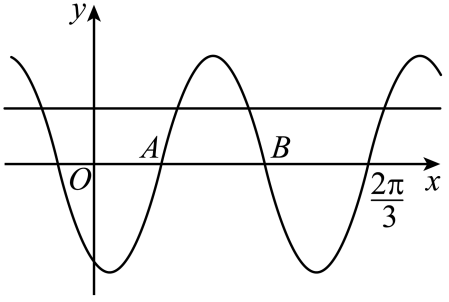
\includegraphics[width=3.5cm]{figures/2023_xgk2_q16.png}\end{tightcenter}
\end{examquestions}

\examsection{四、解答题：本题共6小题，共70分. 解答应写出文字说明、证明过程或演算步骤. }
\begin{examanswers}[start=17]
\item （10分）

记$\triangle ABC$的内角$A,B,C$的对边分别为$a,b,c$，已知$\triangle ABC$的面积为$\sqrt3$，$D$为$BC$中点，且$AD=1$. 

\subq{（1）}{若$\angle ADC=\dfrac\pi3$，求$\tan B$；}

\subq{（2）}{若$b^2+c^2=8$，求$b,c$.}

\item（12分）

$\{a_n\}$为等差数列，$b_n=$\linsys{a_n-6,\quad n \text{为奇数}\\2a_n,\quad\quad n \text{为偶数}}，记$S_n,T_n$分别为数列$\{a_n\}$，$\{b_n\}$的前$n$项和，$S_4=32$，$T_3=16$. 

\subq{（1）}{求$\{a_n\}$的通项公式；}

\subq{（2）}{证明：当$n>5$时，$T_n>S_n$.}

\item（12分）

某研究小组经过研究发现某种疾病的患病者与未患病者的某项医学指标有明显差异，经过大量调查，得到如下的患病者和未患病者该指标的频率分布直方图：

利用该指标制定一个检测标准，需要确定临界值$c$，将该指标大于$c$的人判定为阳性，小于或等于$c$的人判定为阴性. 此检测标准的漏诊率是将患病者判定为阴性的概率，记为$p(c)$；误诊率是将未患病者判定为阳性的概率，记为$q(c)$. 假设数据在组内均匀分布，以事件发生的频率作为相应事件发生的概率. 
\begin{tightcenter}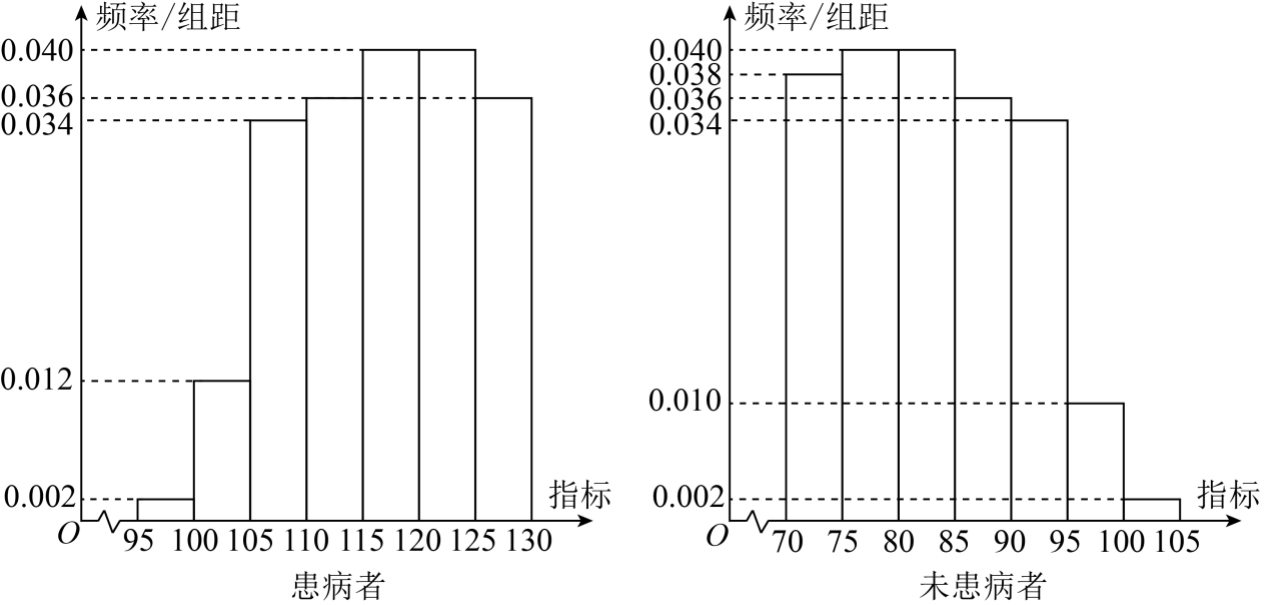
\includegraphics[width=10cm]{figures/2023_xgk2_q19.png}\end{tightcenter}

\subq{（1）}{当漏诊率$p(c)=0.5\%$时，求临界值$c$和误诊率$q(c)$；}

\subq{（2）}{设函数$f(c)=p(c)+q(c)$，当$c\in[95,105]$时，求$f(c)$的解析式，并求$f(c)$在区间$[95,105]$的最小值.}

\item（12分）

如图，三棱锥$A-BCD$中，$DA=DB=DC$，$BD\perp CD$，$\angle ADB=\angle ADC=60^\circ$，$E$为$BC$的中点. 

\noindent\begin{minipage}[t]{0.64\linewidth}
\subq{（1）}{证明：$BC\perp DA$；}

\subq{（2）}{点$F$满足$\vec{EF}=\vec{DA}$，求二面角$D-AB-F$的正弦值.}
\end{minipage}\hfill
\begin{minipage}[t]{0.30\linewidth}
\vspace{-2.5em}
\centering
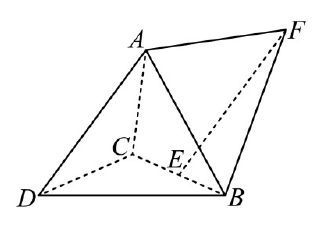
\includegraphics[width=\linewidth]{figures/2023_xgk2_q20.png}
\end{minipage}

\item（12分）

已知双曲线$C$的中心为坐标原点，左焦点为$(-2\sqrt5,0)$，离心率为$\sqrt5$. 

\subq{（1）}{求$C$的方程；}

\subq{（2）}{记$C$的左、右顶点分别为$A_1,A_2$，过点$(-4,0)$的直线与$C$的左支交于$M,N$两点，$M$在第二象限，直线$MA_1$与$NA_2$交于点$P$，证明：点$P$在定直线上.}

\item（12分）

\subq{（1）}{证明：当$0<x<1$时，$x-x^2<\sin x<x$；}

\subq{（2）}{已知函数$f(x)=\cos ax-\ln(1-x^2)$，若$x=0$是$f(x)$的极大值点，求$a$的取值范围.}
\end{examanswers}

\end{document}
